\documentclass[a4paper,11pt]{article}
\usepackage[spanish]{babel} % Para escribir en Espanol normal
\usepackage[utf8]{inputenc}
%\usepackage[latin1]{inputenc}
\usepackage{color}
\usepackage{array}
\usepackage{amsmath,amssymb}
\usepackage{float}
\usepackage{graphicx}
\usepackage{subfig}
\usepackage{enumerate}
\begin{document}

%Portada del Documento
\setlength{\unitlength}{1 cm} %Especificar unidad de trabajo
\thispagestyle{empty}
\begin{picture}(18,4)
\put(1,0){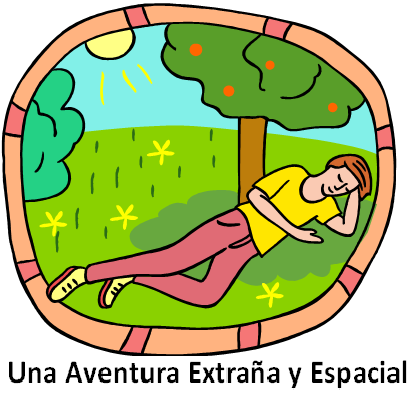
\includegraphics[width=10cm,height=8cm]{apli1.png}}
\end{picture}
\begin{center}
\textbf{{\Huge Proyecto de Python }\\[0.5cm]
{\LARGE Proyecto del Segundo Parcial }}\\[1.25cm]
{\Large Lenguajes de Programación}\\[2.3cm]
{\LARGE \textbf{Manual de Usuario}}\\[3.5cm]
\end{center}
{\Large Integrantes:}
\begin{itemize}

\item Ricardo Campuzano
\item Ana Mora Ocaña
\end{itemize}
\begin{center}
 Ingeniería en Computación\\[0.3cm]
  ESPOL\\[1cm]
Guayaquil - \today
\end{center}
% fin de la portada

%%Tabla de Contenid
\newpage
\tableofcontents
\newpage
\section{ Introducción}

El proyecto realizado con la finalidad de ayudar a personas con discapacidad visual, Interactuando con el usuario por medio de sonido y de instrucciones de voz.
 Consiste en narrar una aventura en la cual nosotros mismos le damos el final dependiendo de las opciones que escojamos,todo esto atravez de instruciones de voz. 
    \subsection{ Requisitos}
\begin{itemize}
\item Instalar Python 2.7.
 \item Instalar la libreria Pygame.
 \item Instalar la libreria Pyaudio.
\item Netbeans 6.9 IDE (no es necesario).
\item Instalar el plugins de Python para netbeans.

\end{itemize}


\begin{figure}[ht!]
 
   \centering
   %%----primera subfigura----
   \subfloat[]{
        \label{fig:pantalla:1}         %% Etiqueta para la primera subfigura
        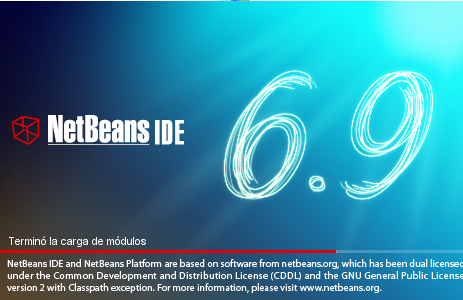
\includegraphics[width=0.42\textwidth]{img1.png}}
   \hspace{0.1\linewidth}
   %%----segunda subfigura----
   \subfloat[]{
        \label{fig:pantalla:2}         %% Etiqueta para la segunda subfigura
        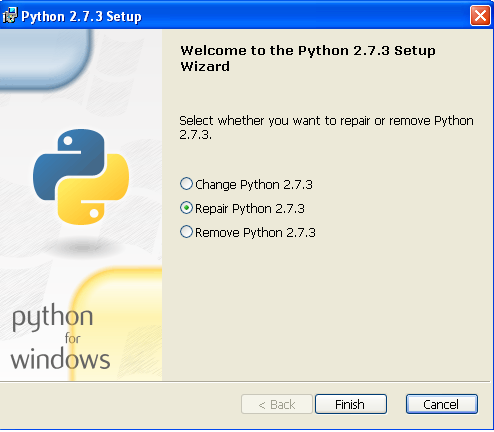
\includegraphics[width=0.42\textwidth]{img2.png}}\\[20pt]
   %%----tercera subfigura----
   \subfloat[]{
        \label{fig:pantalla:3}         %% Etiqueta para la tercera subfigura
        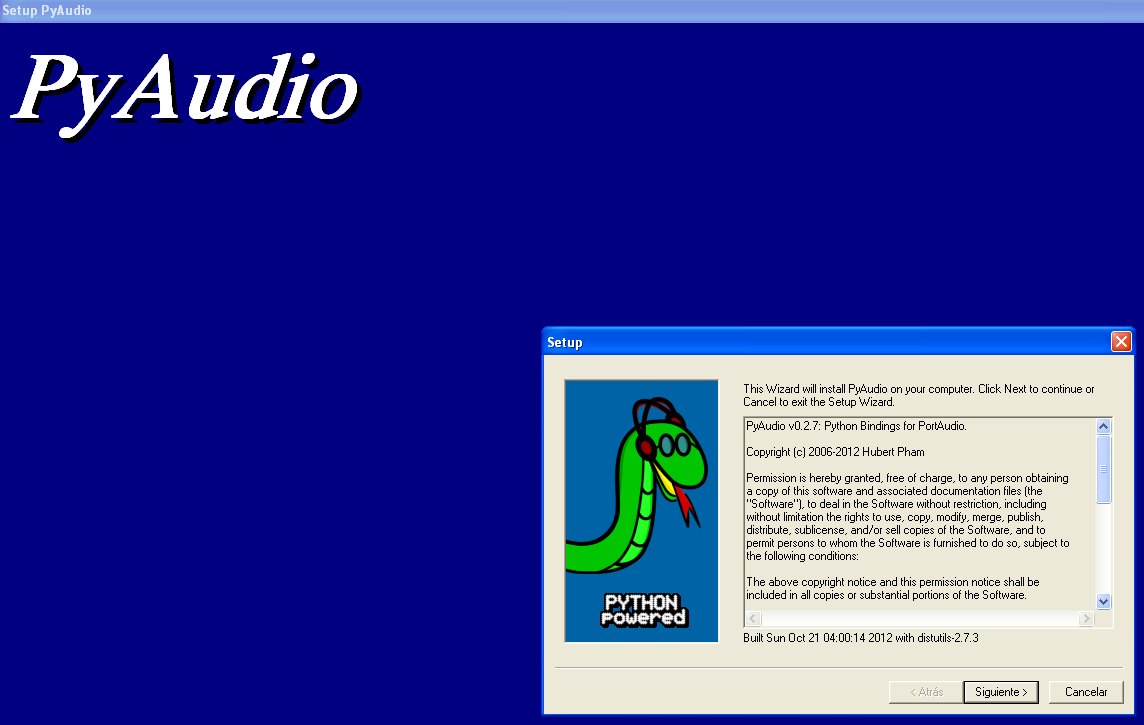
\includegraphics[width=0.42\textwidth]{dibujo.png}}
\hspace{0.1\linewidth}
 %%----cuarta subfigura----
   \subfloat[]{
        \label{fig:pantalla:4}         %% Etiqueta para la tercera subfigura
        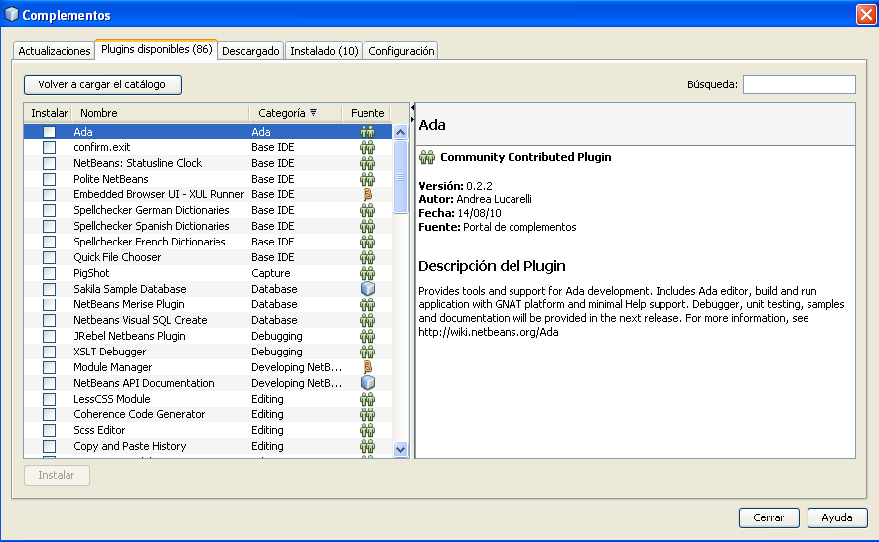
\includegraphics[width=0.42\textwidth]{img3.png}}
    
\end{figure}


\section{ Como ejecutar el proyecto}
Primero copiamos el archivo del proyecto en cualquier directorio, luego abrimos NetBeans , seguimos los siguientes pasos:
\begin{enumerate}
\item Dar click Archivo -> Abrir Proyecto y buscamos la carpeta del proyecto en el directorio que lo guardamos.
\item Luego en la barra de herramientas dar click en ejecutar.
\end{enumerate}
     
\begin{figure}[ht!]
 
   \centering
   %%----primera subfigura----
   \subfloat[]{
        \label{fig:pantalla:1}         %% Etiqueta para la primera subfigura
        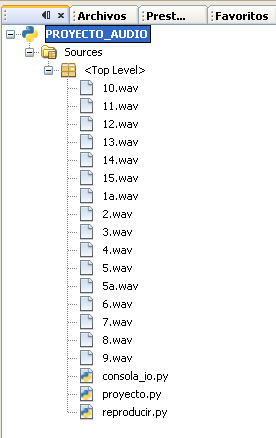
\includegraphics[width=0.42\textwidth]{img4.png}}
   \hspace{0.1\linewidth}
   %%----segunda subfigura----
   \subfloat[]{
        \label{fig:pantalla:2}         %% Etiqueta para la segunda subfigura
        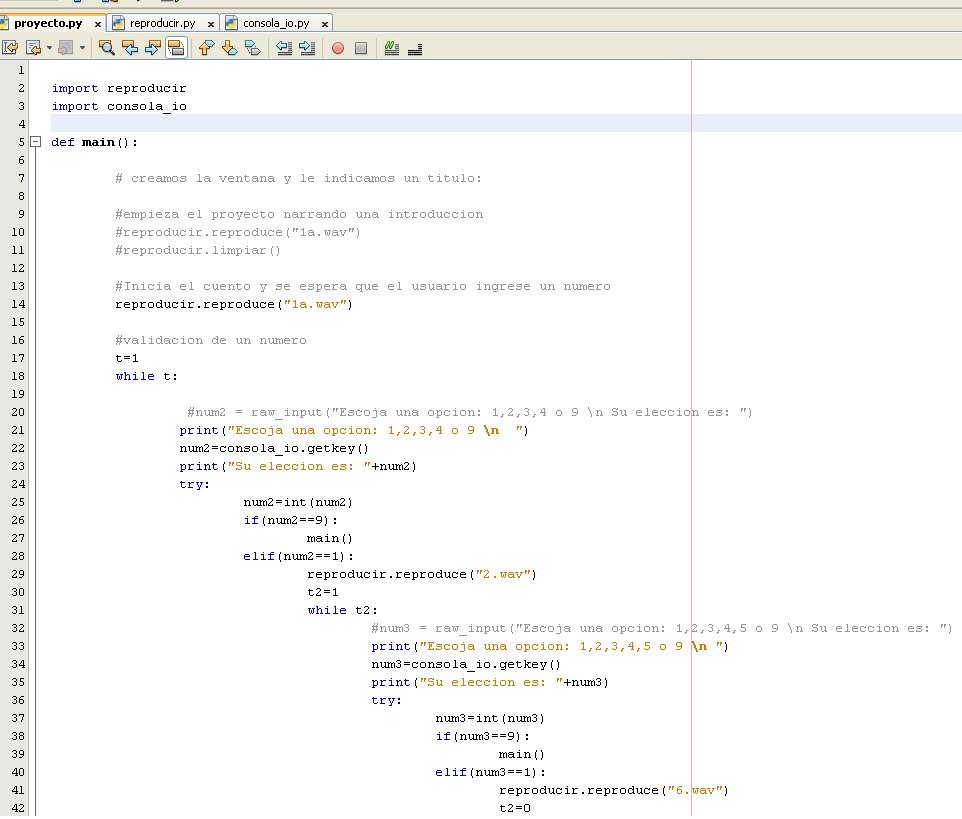
\includegraphics[width=0.42\textwidth]{img5.png}}
\hspace{0.1\linewidth}
   %%----tercera subfigura----
   \subfloat[]{
        \label{fig:pantalla:3}         %% Etiqueta para la tercera subfigura
        
\includegraphics[width=0.42\textwidth]{apli.png}}
\end{figure}

 


\end {document}

